\documentclass[10pt,landscape,letterpaper]{article}
\usepackage{amssymb,amsmath,amsthm,amsfonts}
\usepackage{multicol,multirow}
\usepackage{calc}
\usepackage{ifthen}
\usepackage[landscape]{geometry}
\usepackage[colorlinks=true,citecolor=blue,linkcolor=blue]{hyperref}
\usepackage{fontspec}
\usepackage{xeCJK}
\usepackage{graphicx}
\usepackage{float}
\usepackage{caption}
\usepackage{subcaption}
\usepackage{tikz}
\usepackage{tcolorbox}

\ifthenelse{\lengthtest { \paperwidth = 11in}}
    { \geometry{top=.5in,left=.5in,right=.5in,bottom=.5in} }
	{\ifthenelse{ \lengthtest{ \paperwidth = 297mm}}
		{\geometry{top=1cm,left=1cm,right=1cm,bottom=1cm} }
		{\geometry{top=1cm,left=1cm,right=1cm,bottom=1cm} }
	}
\pagestyle{empty}
\makeatletter
\renewcommand{\section}{\@startsection{section}{1}{0mm}%
                                {-1ex plus -.5ex minus -.2ex}%
                                {0.5ex plus .2ex}%x
                                {\normalfont\large\bfseries}}
\renewcommand{\subsection}{\@startsection{subsection}{2}{0mm}%
                                {-1explus -.5ex minus -.2ex}%
                                {0.5ex plus .2ex}%
                                {\normalfont\normalsize\bfseries}}
\renewcommand{\subsubsection}{\@startsection{subsubsection}{3}{0mm}%
                                {-1ex plus -.5ex minus -.2ex}%
                                {1ex plus .2ex}%
                                {\normalfont\small\bfseries}}
\makeatother
\setcounter{secnumdepth}{0}
\setlength{\parindent}{0pt}
\setlength{\parskip}{0pt plus 0.5ex}
% -----------------------------------------------------------------------

\begin{document}

% \raggedright
\footnotesize

\begin{center}
  \Large{\textbf{Template} } \\
  \footnotesize{Your Name} \\
\end{center}

\begin{multicols}{3}
\setlength{\premulticols}{1pt}
\setlength{\postmulticols}{1pt}
\setlength{\multicolsep}{1pt}
\setlength{\columnsep}{2pt}

\section{}
\begin{quote}
\textit{Less is more.}
\end{quote}

\section{Figures}
\begin{figure}[H]
  \centering
  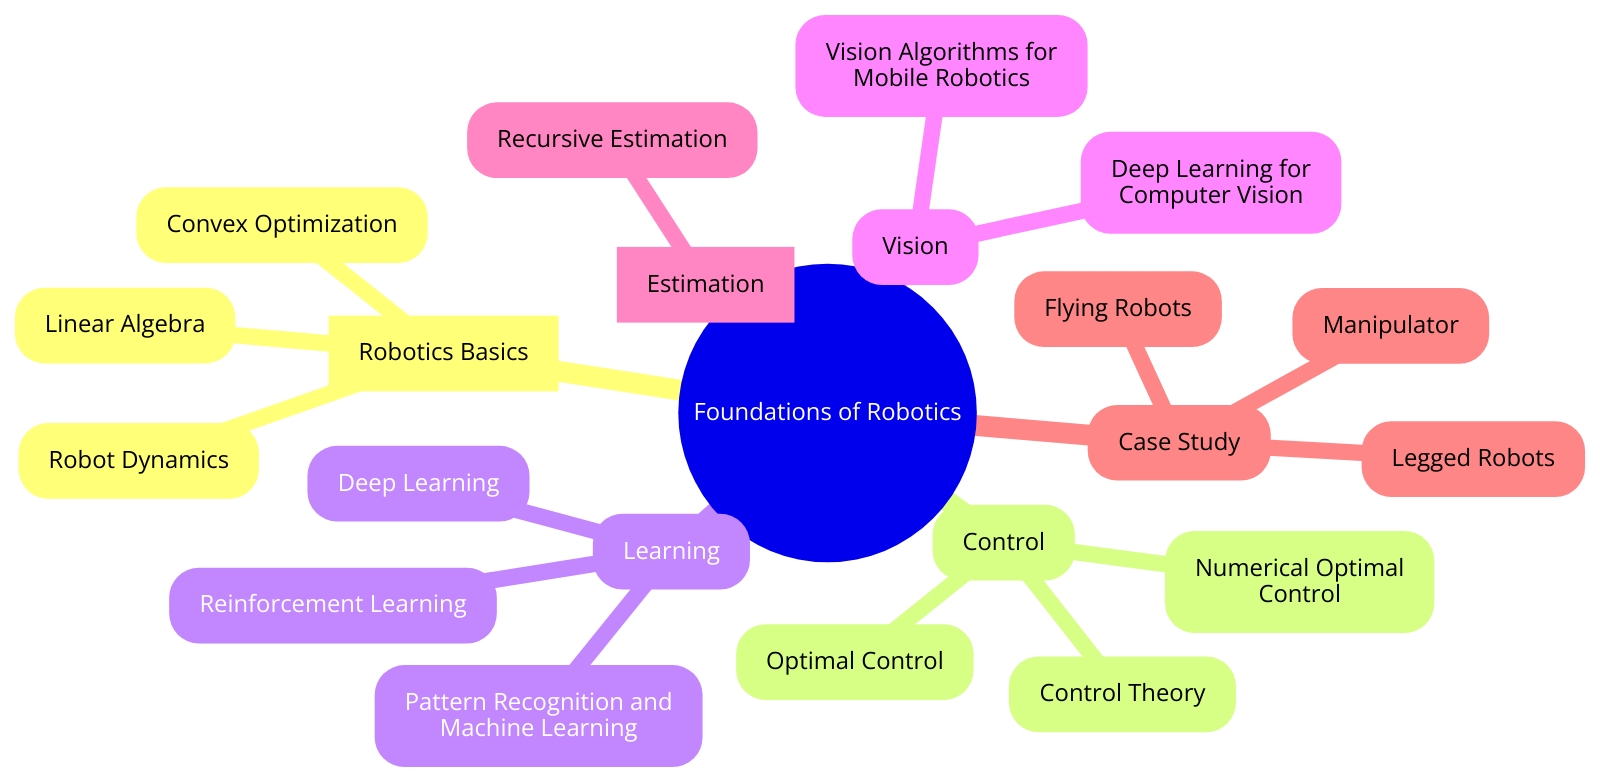
\includegraphics[width=1.0\linewidth]{figures/diagram.png}
  \captionsetup{font=small}
  \caption{Example Image A}
\end{figure}

\section{Color Box}
\begin{tcolorbox}[colback=blue!5!white,colframe=blue!50!black,title=My nice heading]
This is a \textbf{tcolorbox}.
\end{tcolorbox}

\section{Tables}
\begin{table}[H]
  \centering
  \begin{tabular}{c|c|c}
    \hline
    \textbf{Header 1} & \textbf{Header 2} & \textbf{Header 3} \\
    \hline
    1 & 2 & 3 \\
    4 & 5 & 6 \\
    7 & 8 & 9 \\
    \hline
  \end{tabular}
  \caption{Example Table A}
\end{table}

\section{Math}
\begin{align*}
  \min_{x} & \quad f(x) \\
  \text{s.t.} & \quad g(x) \leq 0 \\
\end{align*}

\section{Lists}
\begin{itemize}
  \item Item 1
  \item Item 2
  \item Item 3
\end{itemize}

\section{Code}
\begin{verbatim}
#include <iostream>
using namespace std;

int main() {
  cout << "Hello, World!" << endl;
  return 0;
}
\end{verbatim}

\section{Links}
\begin{itemize}
  \item \href{https://www.google.com}{Google}
  \item \href{https://www.bing.com}{Bing}
\end{itemize}

\end{multicols}
\end{document}

